% "{'classe':('PSI'),'chapitre':'chs_hs','type':('td'),'titre':'Conception de la commande d’un robot chirurgical', 'source':'CCS PSI 2015','comp':[],'corrige':True}"
%\setchapterimage{bandeau}
\chapter*{Colle \arabic{cptColle} \\ 
Conception de la commande d’un robot chirurgical -- 
\ifprof Corrigé \else Sujet \fi}
\addcontentsline{toc}{section}{Colle \arabic{cptColle} :
Conception de la commande d’un robot chirurgical -- 
\ifprof Corrigé \else Sujet \fi}

\iflivret \stepcounter{cptColle} \else
\ifprof  \stepcounter{cptColle} \else \fi
\fi

\setcounter{question}{0}
\marginnote{CCS PSI 2015.}
%\marginnote[1cm]{
%\UPSTIcompetence[2]{C1-02}
%\UPSTIcompetence[2]{C2-04}}

\begin{marginfigure}[4cm]
\centering
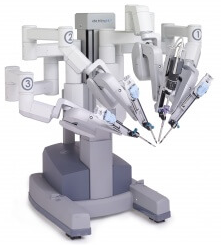
\includegraphics[width=4cm]{fig_00}
\end{marginfigure}







On s'intéresse au bras esclave d'un robot chirurgical. 
\begin{obj}
Justifier la structure du bras esclave par rapport au cahier des charges.
\end{obj}

\begin{center}
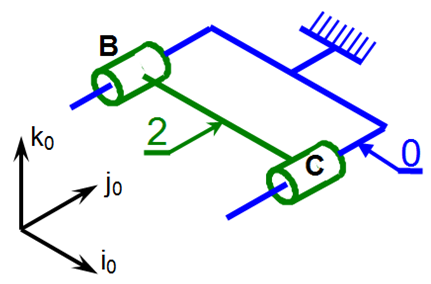
\includegraphics[width=\linewidth]{fig_02.png}
\end{center}

On donne le schéma cinématique partiel du bras esclave.

\begin{center}
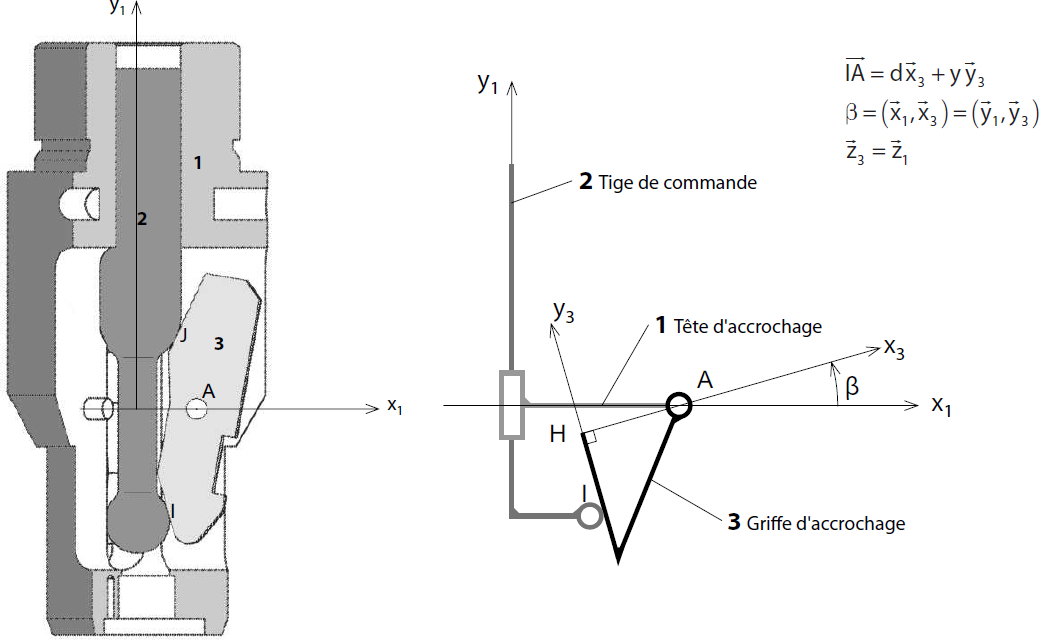
\includegraphics[width=\linewidth]{fig_01.png}
\end{center}

\begin{center}
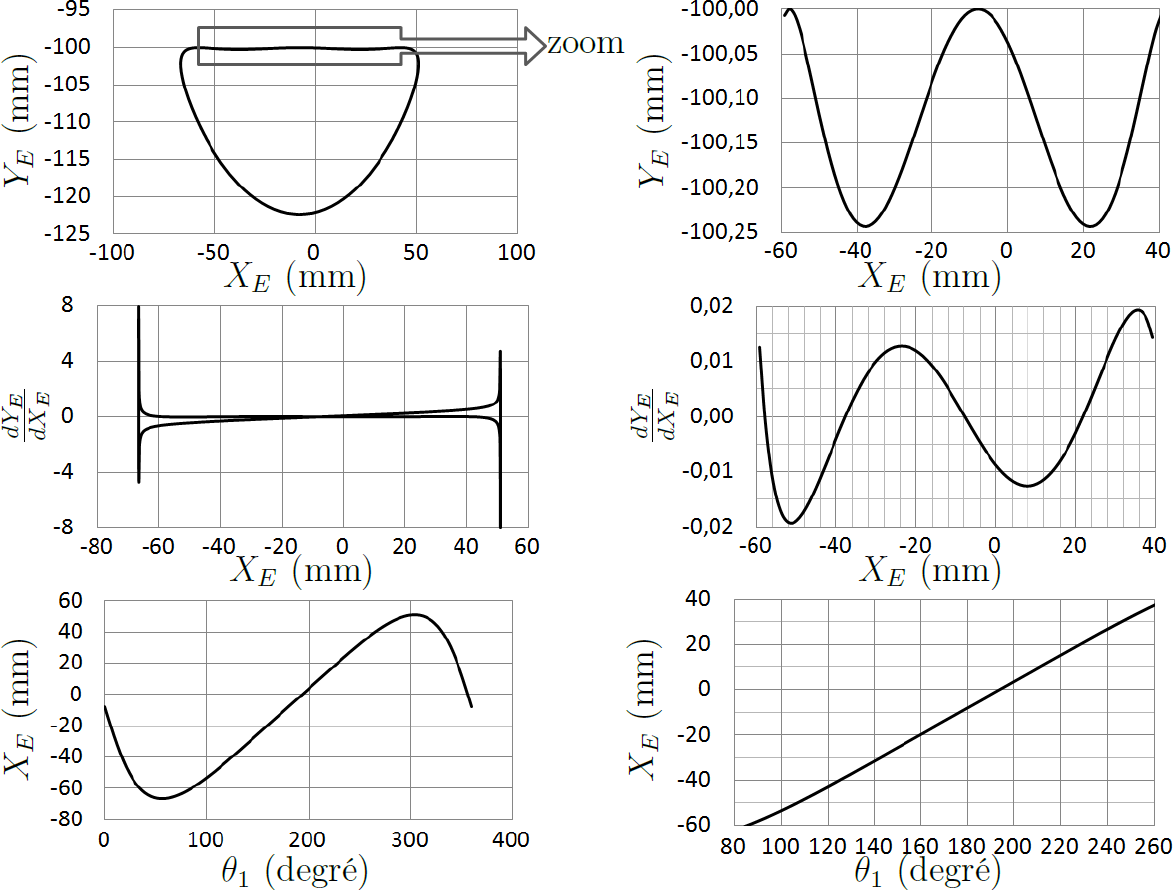
\includegraphics[width=.8\linewidth]{fig_03.png}
\end{center}


\begin{center}
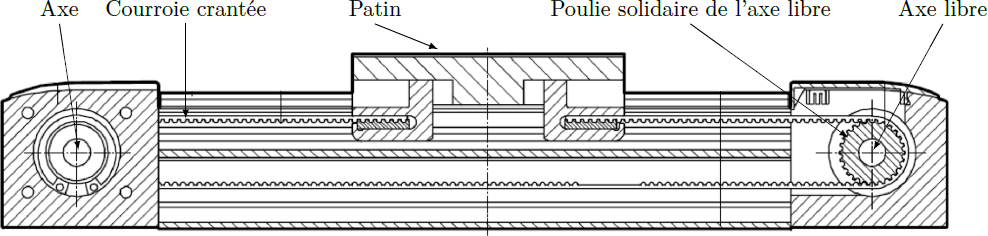
\includegraphics[width=\linewidth]{fig_04.png}
\end{center}

Le point $T$ est situé à l’intersection des axes $\axe{A'}{{x_0}}$ et  $\axe{P'}{{y_2}'}$. 
Le vecteur vitesse du point $T$ de 7’ par rapport à 0, noté $\vectv{T}{7'}{0}$, doit être colinéaire à 
$\vect{y_2}'$.

\question{Tracer le graphe de liaison.}

\question{En s’appuyant sur le schéma cinématique, calculer $\vectv{P}{7'}{0}$ par dérivation du vecteur position.}

\question{Exprimer $\vectv{T}{7'}{0}$ dans la base $\base{x_2'}{y_2'}{z_2'}$ en fonction des données de l’énoncé. Il est conseillé d’utiliser la relation de Varignon en passant par le point $P'$.}


\question{Exprimer le torseur cinématique de $7’/0$ réduit en $T$, par ses composantes dans la base $\base{x_2'}{y_2'}{z_2'}$ et donner la liaison équivalente entre 7’ et 0 au point $T$.}


\question{Quelle exigence du cahier des charges (document réponse) justifie cette structure ? Expliquer sans calcul.}

\question{Mettre à jour le graphe de liaisons et donner le degré d'hyperstatisme du modèle. Vous utiliserez la méthode statique et la méthode cinématique.}

\question{Quel peut être l'avantage de disposer d'un système hyperstatique ?}

\question{En conservant l'architecture du mécanisme, proposer des modifications de liaisons permettant de rendre le modèle isostatique.}

